\chapter{\label{ch:p2} Pràctica P2 -- Accés a l'LCD}

\section{Objectius}

En aquesta pràctica es programarà el mòdul de codi que farà la comunicació
amb l'LCD de la placa, basat en un \emph{driver} HD44780.

Es començarà verificant la compatibilitat a nivell elèctric, llavors
escrivint el codi de baix nivell per fer transferències de 4~bits cap
al LCD. Basant-nos en això, es programaran els mètodes per fer operacions
d'alt nivell al LCD i finalment, uns programes bàsics per demostrar-ne el
seu us.

\section{Desenvolupament}


\subsection{Funcionament de l'LCD}

Aquesta primera part és purament teòrica i explica l'interfície del \emph{driver}
amb el que ens comunicarem, i el seu funcionament a nivell més alt.

A partir d'aquest punt, es farà servir «LCD» per referir-se al driver.


\subsection{Implementació a la placa de pràctiques}

S'expliquen ara les conseqüències de connectar el driver fent servir només 6~línies
en total, que és el cas de la nostra placa, i es donen els esquemàtics corresponents.
Es nota que les 6~línies actuaran en tot moment de sortida de la placa (i entrada
per l'LCD).

Abans d'implementar res, però, es nota també que l'LCD fa servir una alimentació
diferent (\SI{5}{\volt}) a la del microcontrolador (\SI{3}{\volt}) i es demana com
a exercici previ comprovar que els nivells lògics estàtics produits per les
sortides de l'últim son compatibles amb els que espera el primer.

%previ
Segons el datasheet del HD44780U (pàg.~218) i per a \(V_{cc} = \SI{5}{\volt}\),
el nivell baix d'entrada ha d'estar en el rang \SIrange{-0.3}{0.6}{\volt}, i el nivell
alt ha d'estar en el rang \SIrange{2.2}{5}{\volt}.

Segons el datasheet dels STM32F407xx (pàg.~100) per a ports CMOS i assumint \(I_{IO} \leq \SI{8}{\milli\ampere}\),
el nivell baix de sortida està per sota de \SI{0.4}{\volt} i el nivell alt de sortida està per sobre de \SI{2.4}{\volt}.

Per tant, tant el nivell baix (\(\SI{0.4}{\volt} < \SI{0.6}{\volt}\))
com el nivell alt (\(\SI{2.4}{\volt} > \SI{2.2}{\volt}\)) son compatibles, i hi
ha un marge de soroll de \(\pm\SI{200}{\milli\volt}\) en tots dos nivells.
%/previ


\subsection{Codi modular i tipus de dades}

Es demana en primer lloc que s'importin al projecte els dos fitxers \filename{lcd.h} i \filename{lcd.c}
per separar el codi d'accés al LCD de la resta del projecte. Aquests dos fitxers
contenen els prototipus i les definicions (buides) de les funcions que implementarem,
respectivament.

Els dos fitxers donats s'importen i es modifica el Makefile com es demana
(\commit{77c69685b482808d521ca61664bc5b7d6d2f2920}): % TODO: fix overflow

\begin{minted}{diff}
--- a/Makefile
+++ b/Makefile
@@ -21,6 +21,7 @@
 # between Base.c amd main.c
 # The character "\" at the end of all but the last line is important
 PCSRC = Base.c \
+        lcd.c \
         main.c
 
 # COMPILATION OPTIONS ####################################################
\end{minted}
\vskip -1em

Comprovem que en tornar a compilar, ja es genera el fitxer objecte \filename{lcd.o} a \filename{build/obj}.

També afegim l'inclusió de \filename{lcd.h} a \filename{main.c}:

\begin{minted}{diff}
--- a/main.c
+++ b/main.c
@@ -7,6 +7,7 @@
  *************************************************************/
 
 #include "Base.h"     // Basic definitions
+#include "lcd.h"      // LCD module header file
 
 // Function that blinks the green LED
 
\end{minted}
\vskip -1em

A continuació s'aprofundeix en convencions del codi, com els tipus que es faran
servir i el tamany de cadascun, i la separació de funcions.


\subsection{Configuració dels ports}

Comença ara la implementació de codi en sí. La part divertida! Per començar es
demana programar les 7 línies associades al LCD (6 pel driver, 1 pel backlight)
com a sortida, ja que per defecte el codi d'inicialització les deixa en mode
entrada (per seguretat).

Seguint les explicacions sobre la configuració de les línies GPIO, i les
indicacions per al nostre cas concret (amb \SI{2}{\mega\hertz} n'hi ha prou
per a la velocitat), cal fer el codi per configurar totes les línies de l'LCD
com a sortides push-pull (funció \fname{lcdGPIOInit}).

\opcional
No obstant, se segueix la recomanació de l'apartat opcional i s'elabora una funció
genèrica per posar un port arbitrari en mode push-pull, que a més no depen de
l'estat del port. Aquesta funció s'anomenarà \fname{GPIO_ModePushPull}:

\begin{minted}{c}
// Configure a GPIO line as push-pull output, at the lowest speed,
// and write a low value
//     port: GPIO port
//     line: GPIO line to set as output
void GPIO_ModePushPull(GPIO_TypeDef *port, int32_t line) {
    // MODERy[1:0] -> 01 General purpose output mode
    port->MODER = (port->MODER & ~(0b11 << line * 2)) | (0b01 << line * 2);

    // OTy -> 0 Push-pull output
    port->OTYPER = (port->OTYPER & ~(0b1 << line)) | (0b0 << line);

    // OSPEEDRy[1:0] -> 00 Speed 25MHz
    port->OSPEEDR = (port->OSPEEDR & ~(0b11 << line * 2)) | (0b00 << line * 2);

    // PUPDRy[1:0] -> 00 No pull-up, no pull-down
    port->PUPDR = (port->PUPDR & ~(0b11 << line * 2)) | (0b00 << line * 2);

    // ODRy -> 0
    port->ODR = (port->ODR & ~(0b1 << line)) | (0b0 << line);
}
\end{minted}
\vskip -1em

\voluntari
Per mantenir el codi ordenat i modular, s'ha generat un parell de fitxers \filename{util.h}
i \filename{util.c} basant-se en l'estructura de \filename{lcd.h} i \filename{lcd.c}, on
s'aniran depositant aquestes utilitats genèriques que puguin ser d'us per altres mòduls.
Un cop definida la funció en aquests dos fitxers, s'ha afegit \filename{util.c} al \filename{Makefile}
tal i com hem fet anteriorment. El parell de fitxers i aquest últim canvi conformen el
\commit{0b5a6be54c882e027bb5083825d6bdefcb2d45ea}.

Seguint amb la pràctica, s'ha definit la funció \fname{lcdGPIOInit} fent us de l'utilitat
definida (estudi previ):

%previ
\begin{minted}{c}
static void lcdGPIOInit(void) {
    GPIO_ModePushPull(LCD_PORT, LCD_BL_PAD);
    GPIO_ModePushPull(LCD_PORT, LCD_E_PAD);
    GPIO_ModePushPull(LCD_PORT, LCD_RS_PAD);
    GPIO_ModePushPull(LCD_PORT, LCD_DB4_PAD);
    GPIO_ModePushPull(LCD_PORT, LCD_DB5_PAD);
    GPIO_ModePushPull(LCD_PORT, LCD_DB6_PAD);
    GPIO_ModePushPull(LCD_PORT, LCD_DB7_PAD);
}
\end{minted}
\vskip -1em
%/previ

Aquesta codi s'ha insertat a \filename{lcd.c} junt amb la inclusió de \filename{util.c}:

\begin{minted}{diff}
--- a/lcd.c
+++ b/lcd.c
@@ -8,6 +8,7 @@
 
 #include "Base.h"  // Basic definitions
 #include "lcd.h"   // LCD definitions
+#include "util.h"
 
 // Some of the function need to be completed
 // as is requested on the manual
\end{minted}
\vskip -1em

Per brevetat, a partir d'aquest punt no es mencionaran les inclusions de \emph{headers}.


\subsection{Gestió del backlight}

S'explica el que és la llum de \emph{backlight} i el pin que permet controlar-la.
Llavors es demana com a estudi previ, fer el codi de la funció \fname{LCD_Backlight}
que encen o apaga el backlight si el seu argument és cert o fals, respectivament.

%previ
\begin{minted}{c}
// Backlight configuration
//     on evaluates to TRUE   Turn on backlight
//     on evaluates to FALSE  Turn off backlight

void LCD_Backlight(int32_t on) {
    if (on)
        LCD_PORT->BSRR.H.set = LCD_BL_BIT;
    else
        LCD_PORT->BSRR.H.clear = LCD_BL_BIT;
}
\end{minted}
\vskip -1em
%/previ

El codi de la funció s'emplena a \filename{lcd.c}. Llavors es demana provar el següent
programa donat per verificar les funcions \fname{lcdGPIOInit} i \fname{LCD_Backlight}:

\begin{minted}{c}
int main(void) {
    baseInit();         // Basic initialization
    LCD_Init();         // Initializes the LCD
    LCD_Backlight(1);   // Turn on LCD backlight
    SLEEP_MS(2000);     // Wait 2s
    LCD_Backlight(0);   // Turn off LCD backlight
    while (1);          // Infinite loop so we don't exit main()
}
\end{minted}
\vskip -1em

La funció \fname{LCD_Init}, entre altres coses conté una crida a \fname{lcdGPIOInit}.
Carreguem el codi a la placa i comprovem que té el funcionament esperat (el backlight
s'encen durant dos segons, i s'apaga). En la figura~\ref{fig:p2-board-backlight} es
pot veure la placa amb el backlight encès.

\begin{figure}
  \begin{center}
    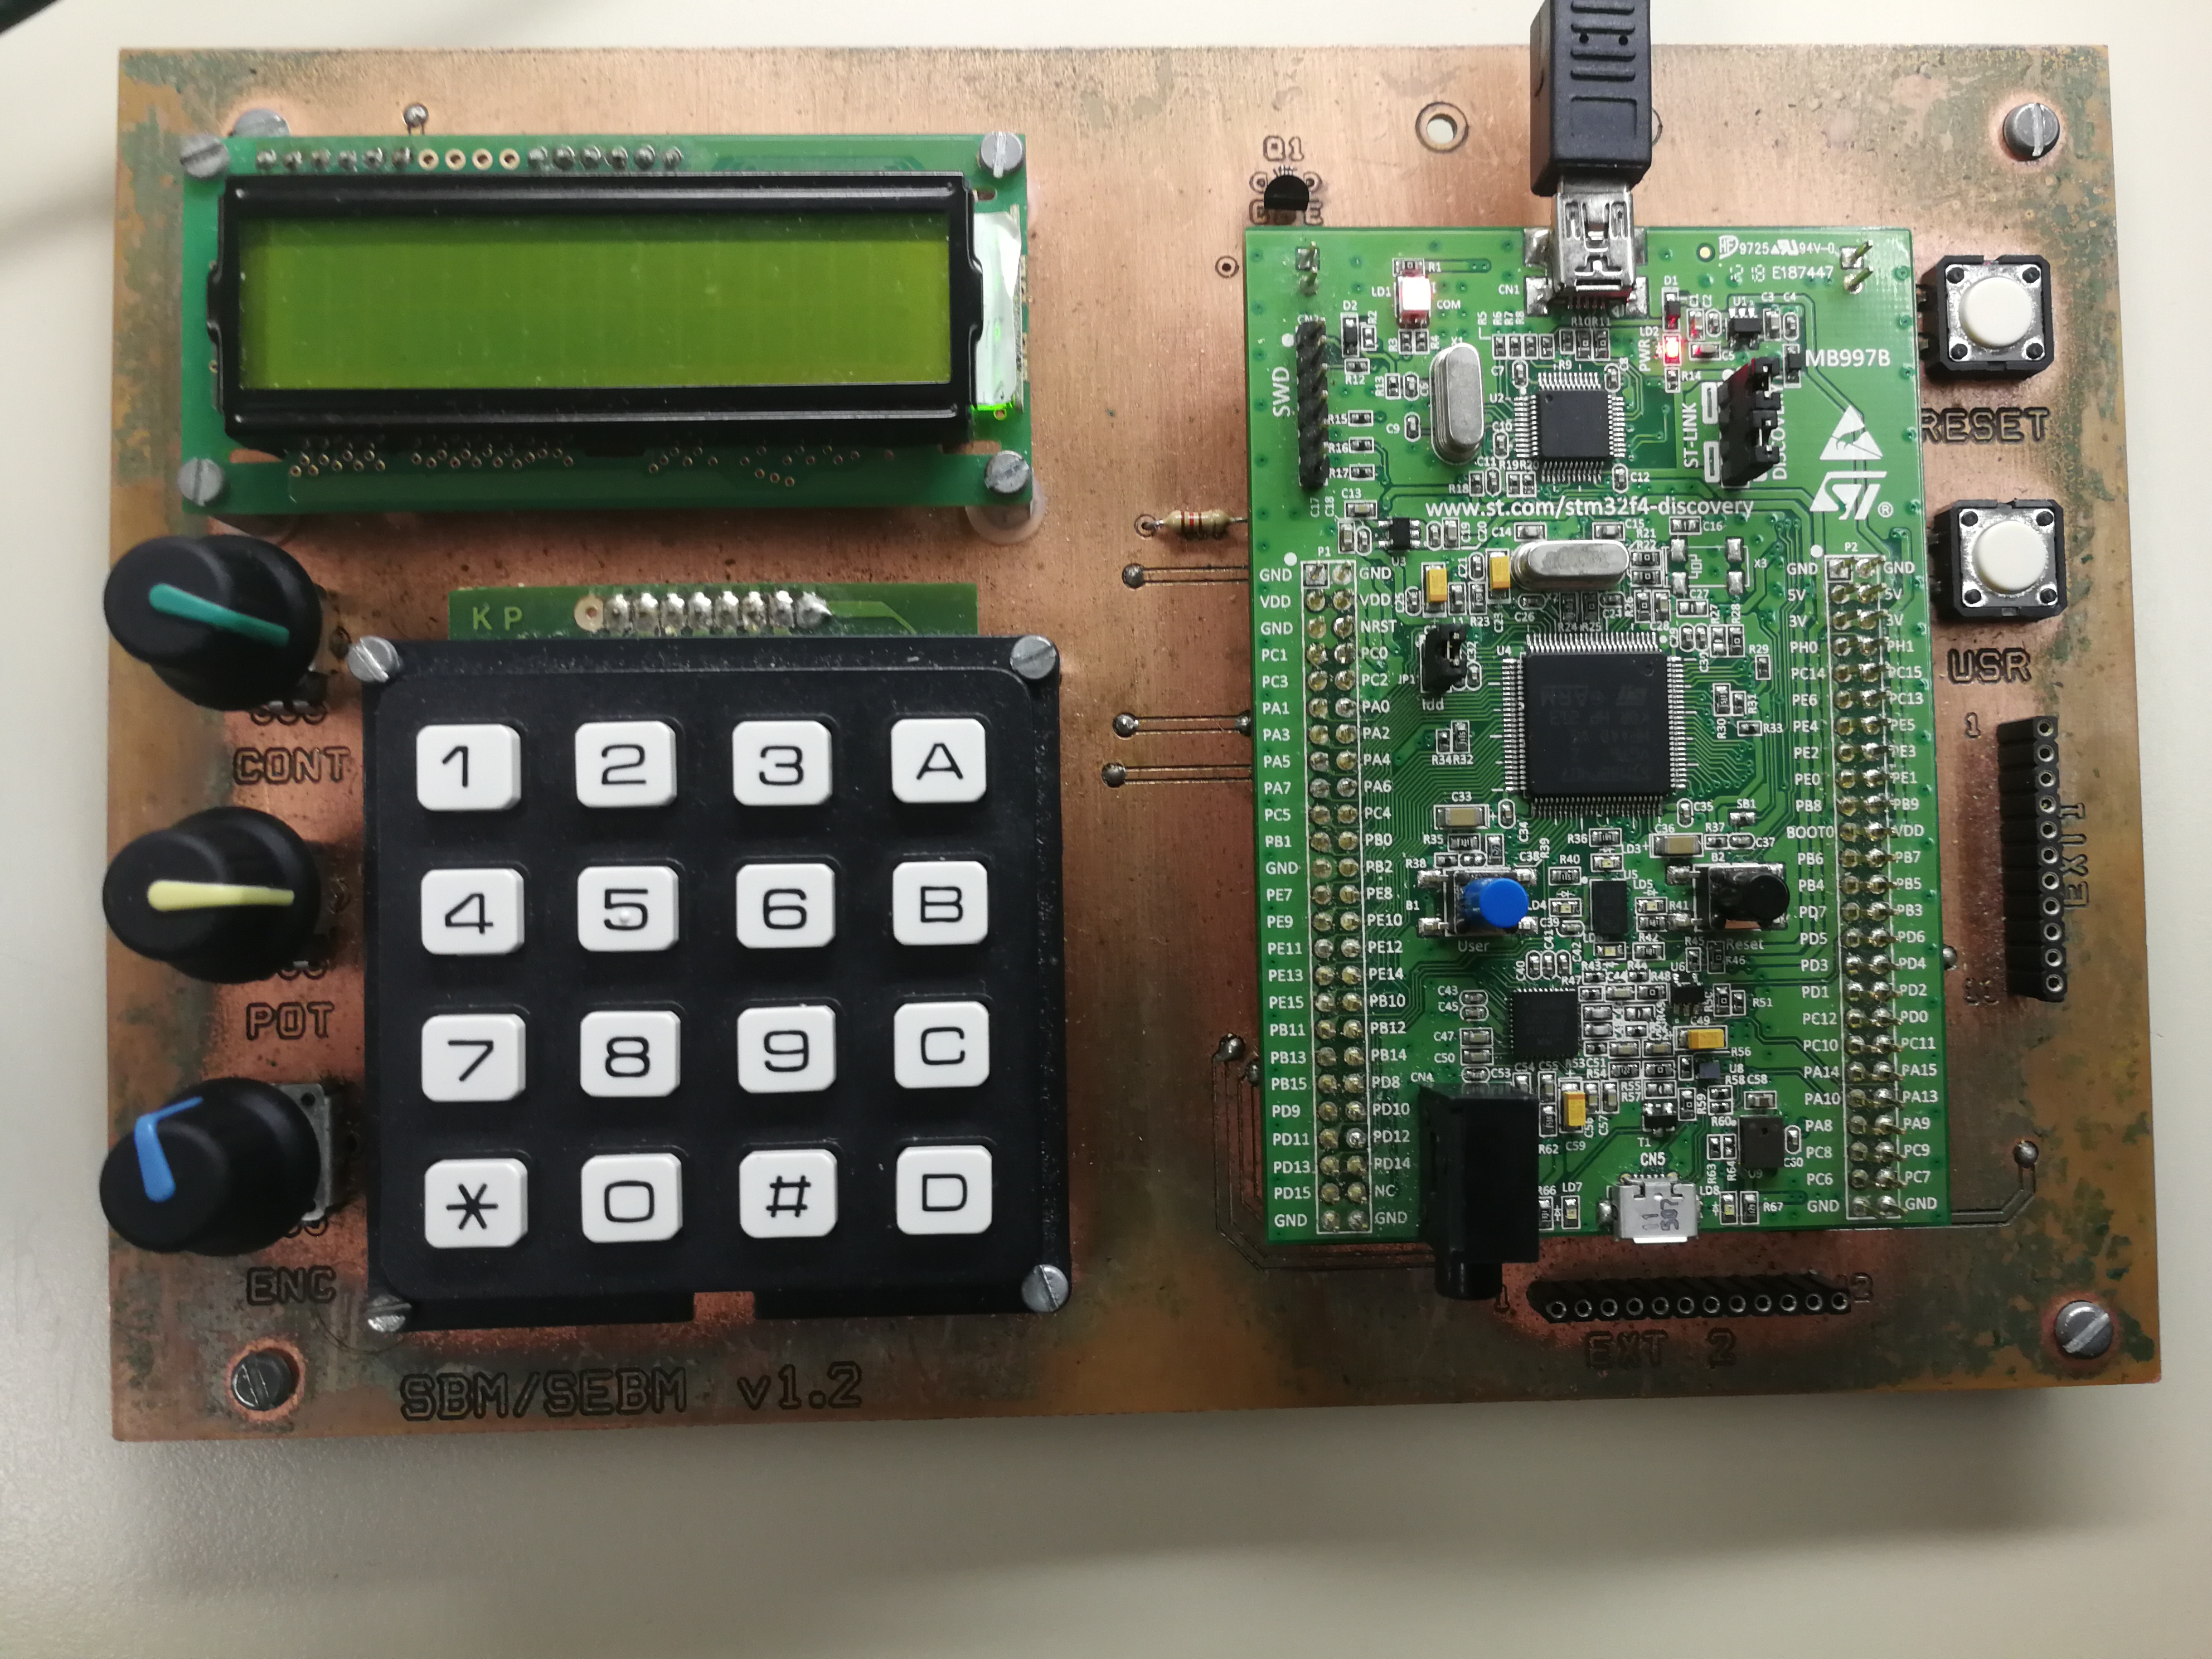
\includegraphics[width=1\columnwidth]{../photos/board/p2-backlight}
  \end{center}
  \caption{ \label{fig:p2-board-backlight} La placa amb el backlight encès. }
\end{figure}


\subsection{\label{sub:p2-init} Inicialització del display}

En aquest pas s'explica la seqüència d'inicialització que cal dur a terme a l'LCD.
Com que l'LCD arrenca en mode 8~bits, cal fer una seqüència d'inicialització
concreta per posar-lo en mode 4~bits i configurar les línies del display i la font.

\begin{figure}
  \begin{center}
    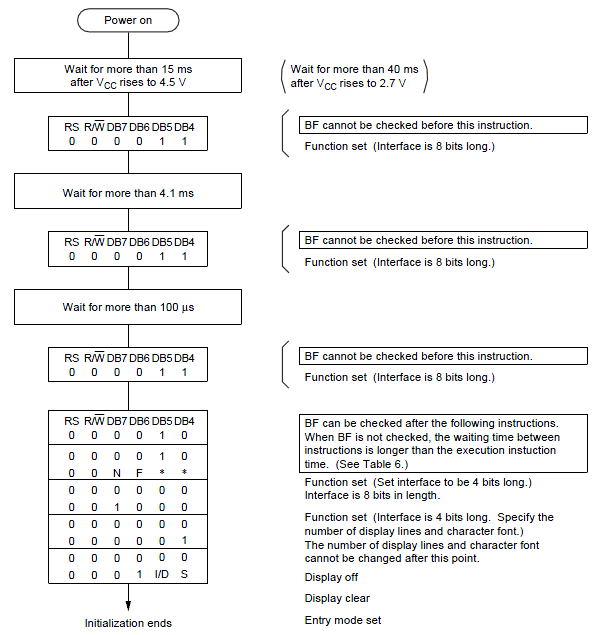
\includegraphics[width=0.8\columnwidth]{../\projectname/lcd-init-protocol}
  \end{center}
  \caption{ \label{fig:p2-init-protocol} Passos d'inicialització de l'LCD en mode 4~bits. }
\end{figure}

Els passos d'aquesta inicialització es poden veure en la figura~\ref{fig:p2-init-protocol}
i ja estan programats en la funció \fname{LCD_Init} que hem cridat abans,
però fa crides a una funció \fname{lcdNibble} que es dona buida:

\begin{minted}{c}
void lcdNibble(int32_t nibbleCmd, int32_t RS)
\end{minted}
\vskip -1em

Aquesta funció hauria de fer una única transferència de 4~bits (donats pels bits més baixos
de \mintinline{c}|nibbleCmd|) tal i com s'indica en el cronograma del datasheet del LCD,
que es pot veure a la figura~\ref{fig:p2-timing-write}.
Cal tenir en compte que, a causa de la connexió de 6~línies que s'ha mencionat,
$\mathsf{R}/\overline{\mathsf{W}}$ està fixat sempre a 0 (escritura) i que les línies
\textsf{DB4} a \textsf{DB7} estan fixades també a 0.

\begin{figure}
  \begin{center}
    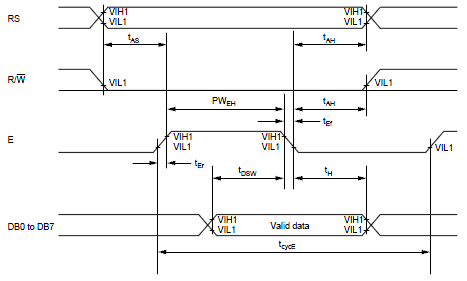
\includegraphics[width=1\columnwidth]{../\projectname/timing-lcd-write}
  \end{center}
  \caption{ \label{fig:p2-timing-write} Cronograma d'una escriptura al LCD. }
\end{figure}

Implementem aquesta funció com es demana (estudi previ):

%previ
\begin{minted}[mathescape]{c}

// Send 4 bits to the LCD and generates an enable pulse
//     nibbleCmd : Bits 3..0 Nibble to send to DB7...DB4
//     RS        : TRUE (RS="1")   FALSE (RS="0")

static void lcdNibble(uint32_t nibbleCmd, int32_t RS) {
    // Set RS and DB4..DB7 and sleep 10us
    LCD_PORT->BSRR.H.set = (nibbleCmd & 0b1111) << LCD_DB4_PAD | (RS ? LCD_RS_BIT : 0);
    LCD_PORT->BSRR.H.clear = (~nibbleCmd & 0b1111) << LCD_DB4_PAD | (!RS ? LCD_RS_BIT : 0);
    DELAY_US(10);
    // Enable E for $\SI{10}{\micro\second}$
    LCD_PORT->BSRR.H.set = LCD_E_BIT;
    DELAY_US(10);
    // Disable E and wait another $\SI{10}{\micro\second}$
    LCD_PORT->BSRR.H.clear = LCD_E_BIT;
    DELAY_US(10);
}
\end{minted}
\vskip -1em
%/previ

Insertem el contingut de la funció a \filename{lcd.c} i ara canviem el programa
de \filename{main.c} de tal forma que es limiti a cridar \fname{LCD_Init}:

\begin{minted}{c}
int main(void) {
    baseInit();         // Basic initialization
    LCD_Init();         // Program the GPIO I/O lines
    while (1);          // Infinite loop so we don't exit main()
}
\end{minted}
\vskip -1em

Si tot ha funcionat bé hauriem de veure \texttt{OK} a la pantalla, ja que després
de la inicialització en sí, \fname{LCD_Init} escriu aquests dos caràcters.

El programa es carrega a la placa i s'obté el funcionament esperat (figura~\ref{fig:p2-board-init}).

\begin{figure}
  \begin{center}
    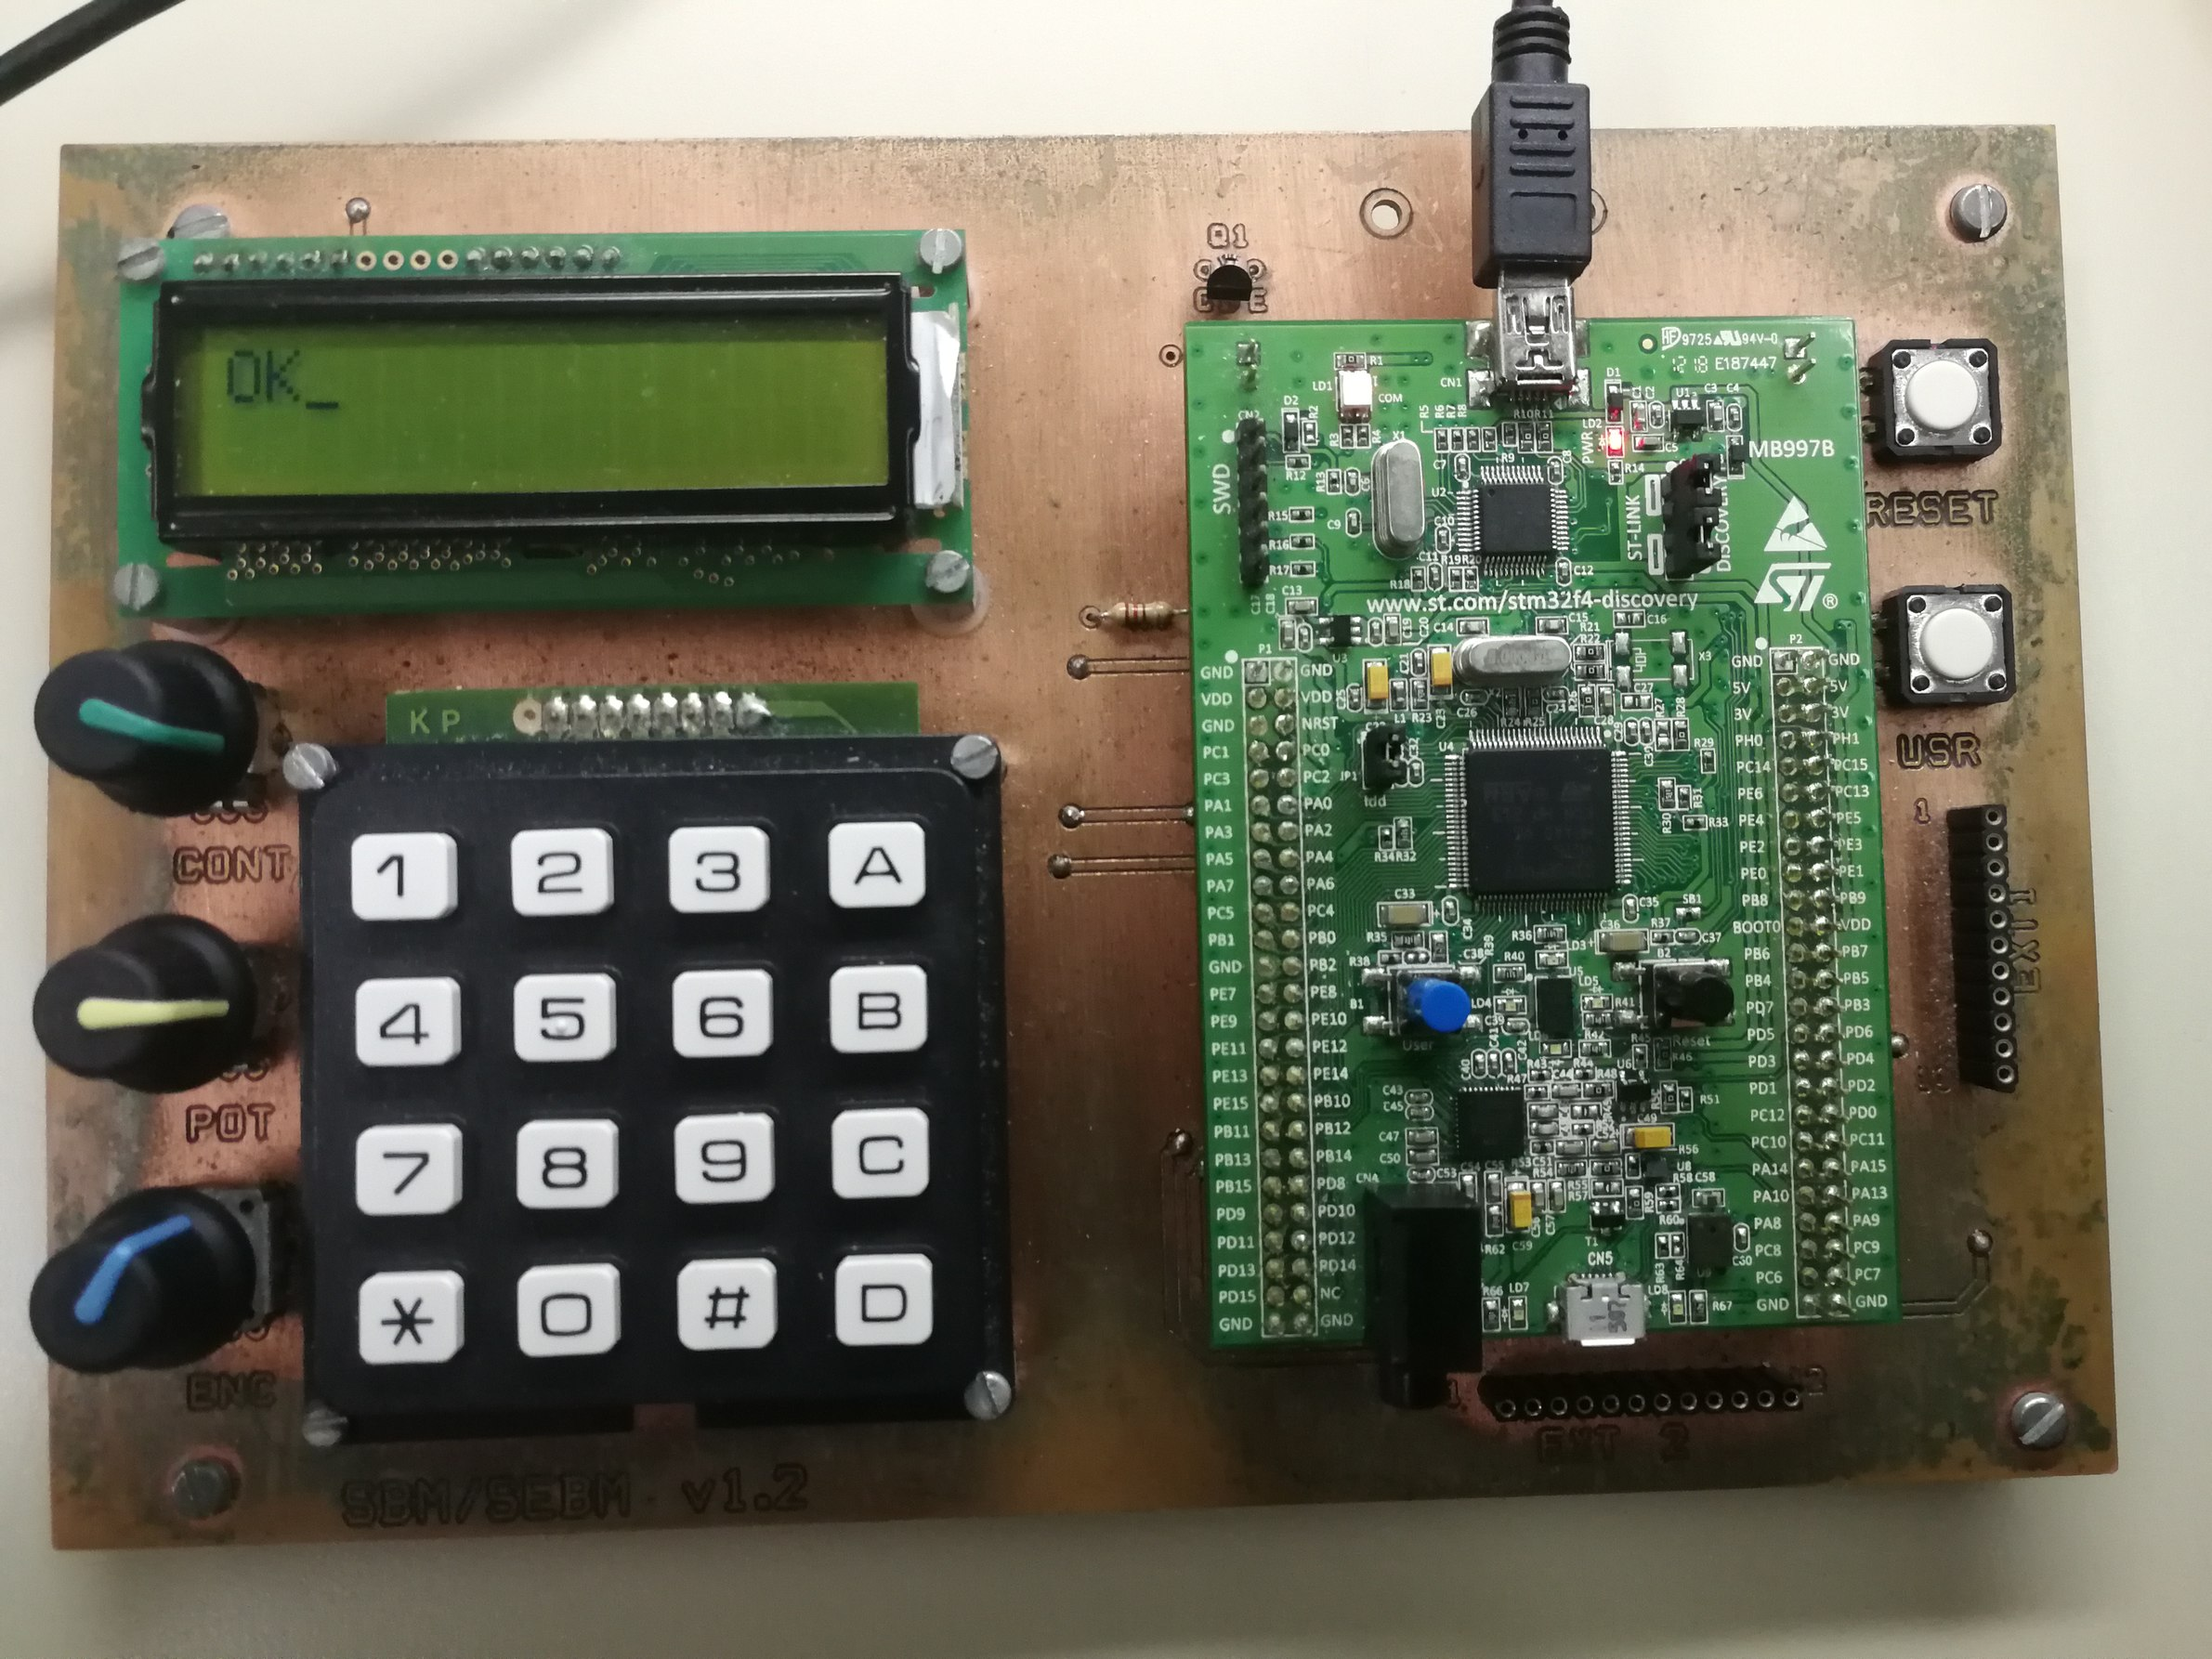
\includegraphics[width=1\columnwidth]{../photos/board/p2-init}
  \end{center}
  \caption{ \label{fig:p2-board-init} La placa just després d'inicialitzar el LCD. }
\end{figure}

Més endavant, en la pràctica P4 es mesurarà i verificarà (pàgina~\pageref{sub:p4-lcd})
que les escritures i el procés d'inicialització en general es fa bé.


\subsection{Escrivint text al display i altres funcions}

S'explica el procés d'escritura a la DDRAM per mostrar caràcters a la pantalla,
i el fet que, com que estem en mode 4~bits, un byte s'escriu primer transferint
els quatre bits alts mitjançant \fname{lcdNibble}, i després els quatre bits
baixos mitjançant la mateixa funció.

\voluntari
Per simplificar el codi, i com que un cop feta la inicialització \fname{lcdNibble}
sempre es cridarà de dos en dos, s'ha fet una funció intermèdia \fname{lcdValue}
també estàtica que escriu un byte fent primer la transferència dels bits alts i
després dels baixos:

\begin{minted}{c}
// Send a full 8-bit value to the LCD by first writing the higher nibble
// and then the lower nibble

static inline void lcdValue(uint32_t cmd, int32_t RS) {
    lcdNibble((cmd >> 4) & 0xF, RS);
    lcdNibble(cmd & 0xF, RS);
}
\end{minted}
\vskip -1em

A més de simplificar el codi que s'escriurà a continuació, això permet canviar fàcilment
cap al mode 8~bits ja que només caldria modificar \fname{lcdValue}.

Seguint amb la pràctica, es demana com a estudi previ implementar la funció
\fname{LCD_SendChar} que haurà d'escriure un caràcter a la DDRAM (suposant que
l'address counter ja està posicionat on es desitja). La implementació d'aquest
mètode és molt simple, només cal fer una escritura amb $\mathsf{RS} = 1$ i
fer l'espera que demana la datasheet per garantitzar que l'operació s'acaba:

%previ
\begin{minted}{c}
// Send a character to the LCD at the current position
//     car: Charater to send

void LCD_SendChar(char car) {
    lcdValue(car, 1);
    DELAY_US(40);
}
\end{minted}
\vskip -1em
%/previ

La funció \fname{LCD_SendString} només ha de cridar \fname{LCD_SendChar} per
cada caràcter de l'string:

%previ
\begin{minted}{c}
// Send a string to the LCD at the current position
//     string: String to send

void LCD_SendString(char *string) {
    // Send every character except the NUL terminator
    for (; *string != '\0'; string++)
        LCD_SendChar(*string);
}
\end{minted}
\vskip -1em
%/previ

La primera funció ja implementa l'espera necessària després de cada escritura, per
tant no cal fer-la en la segona.

Tal i com es suggereix al manual, es modifica el programa a \filename{main.c} per afegir una crida
\mintinline[breakbytokenanywhere=true, breakbytoken=true, breaklines=true]{c}|LCD_SendString("Hello");| després de la inicialització de l'LCD.
El codi es carrega a la placa i es comprova que s'obté el funcionament esperat
(figure~\ref{fig:p2-board-hello}), amb l'LCD mostrant \texttt{OKHello} i el
cursor actiu.

\begin{figure}
  \begin{center}
    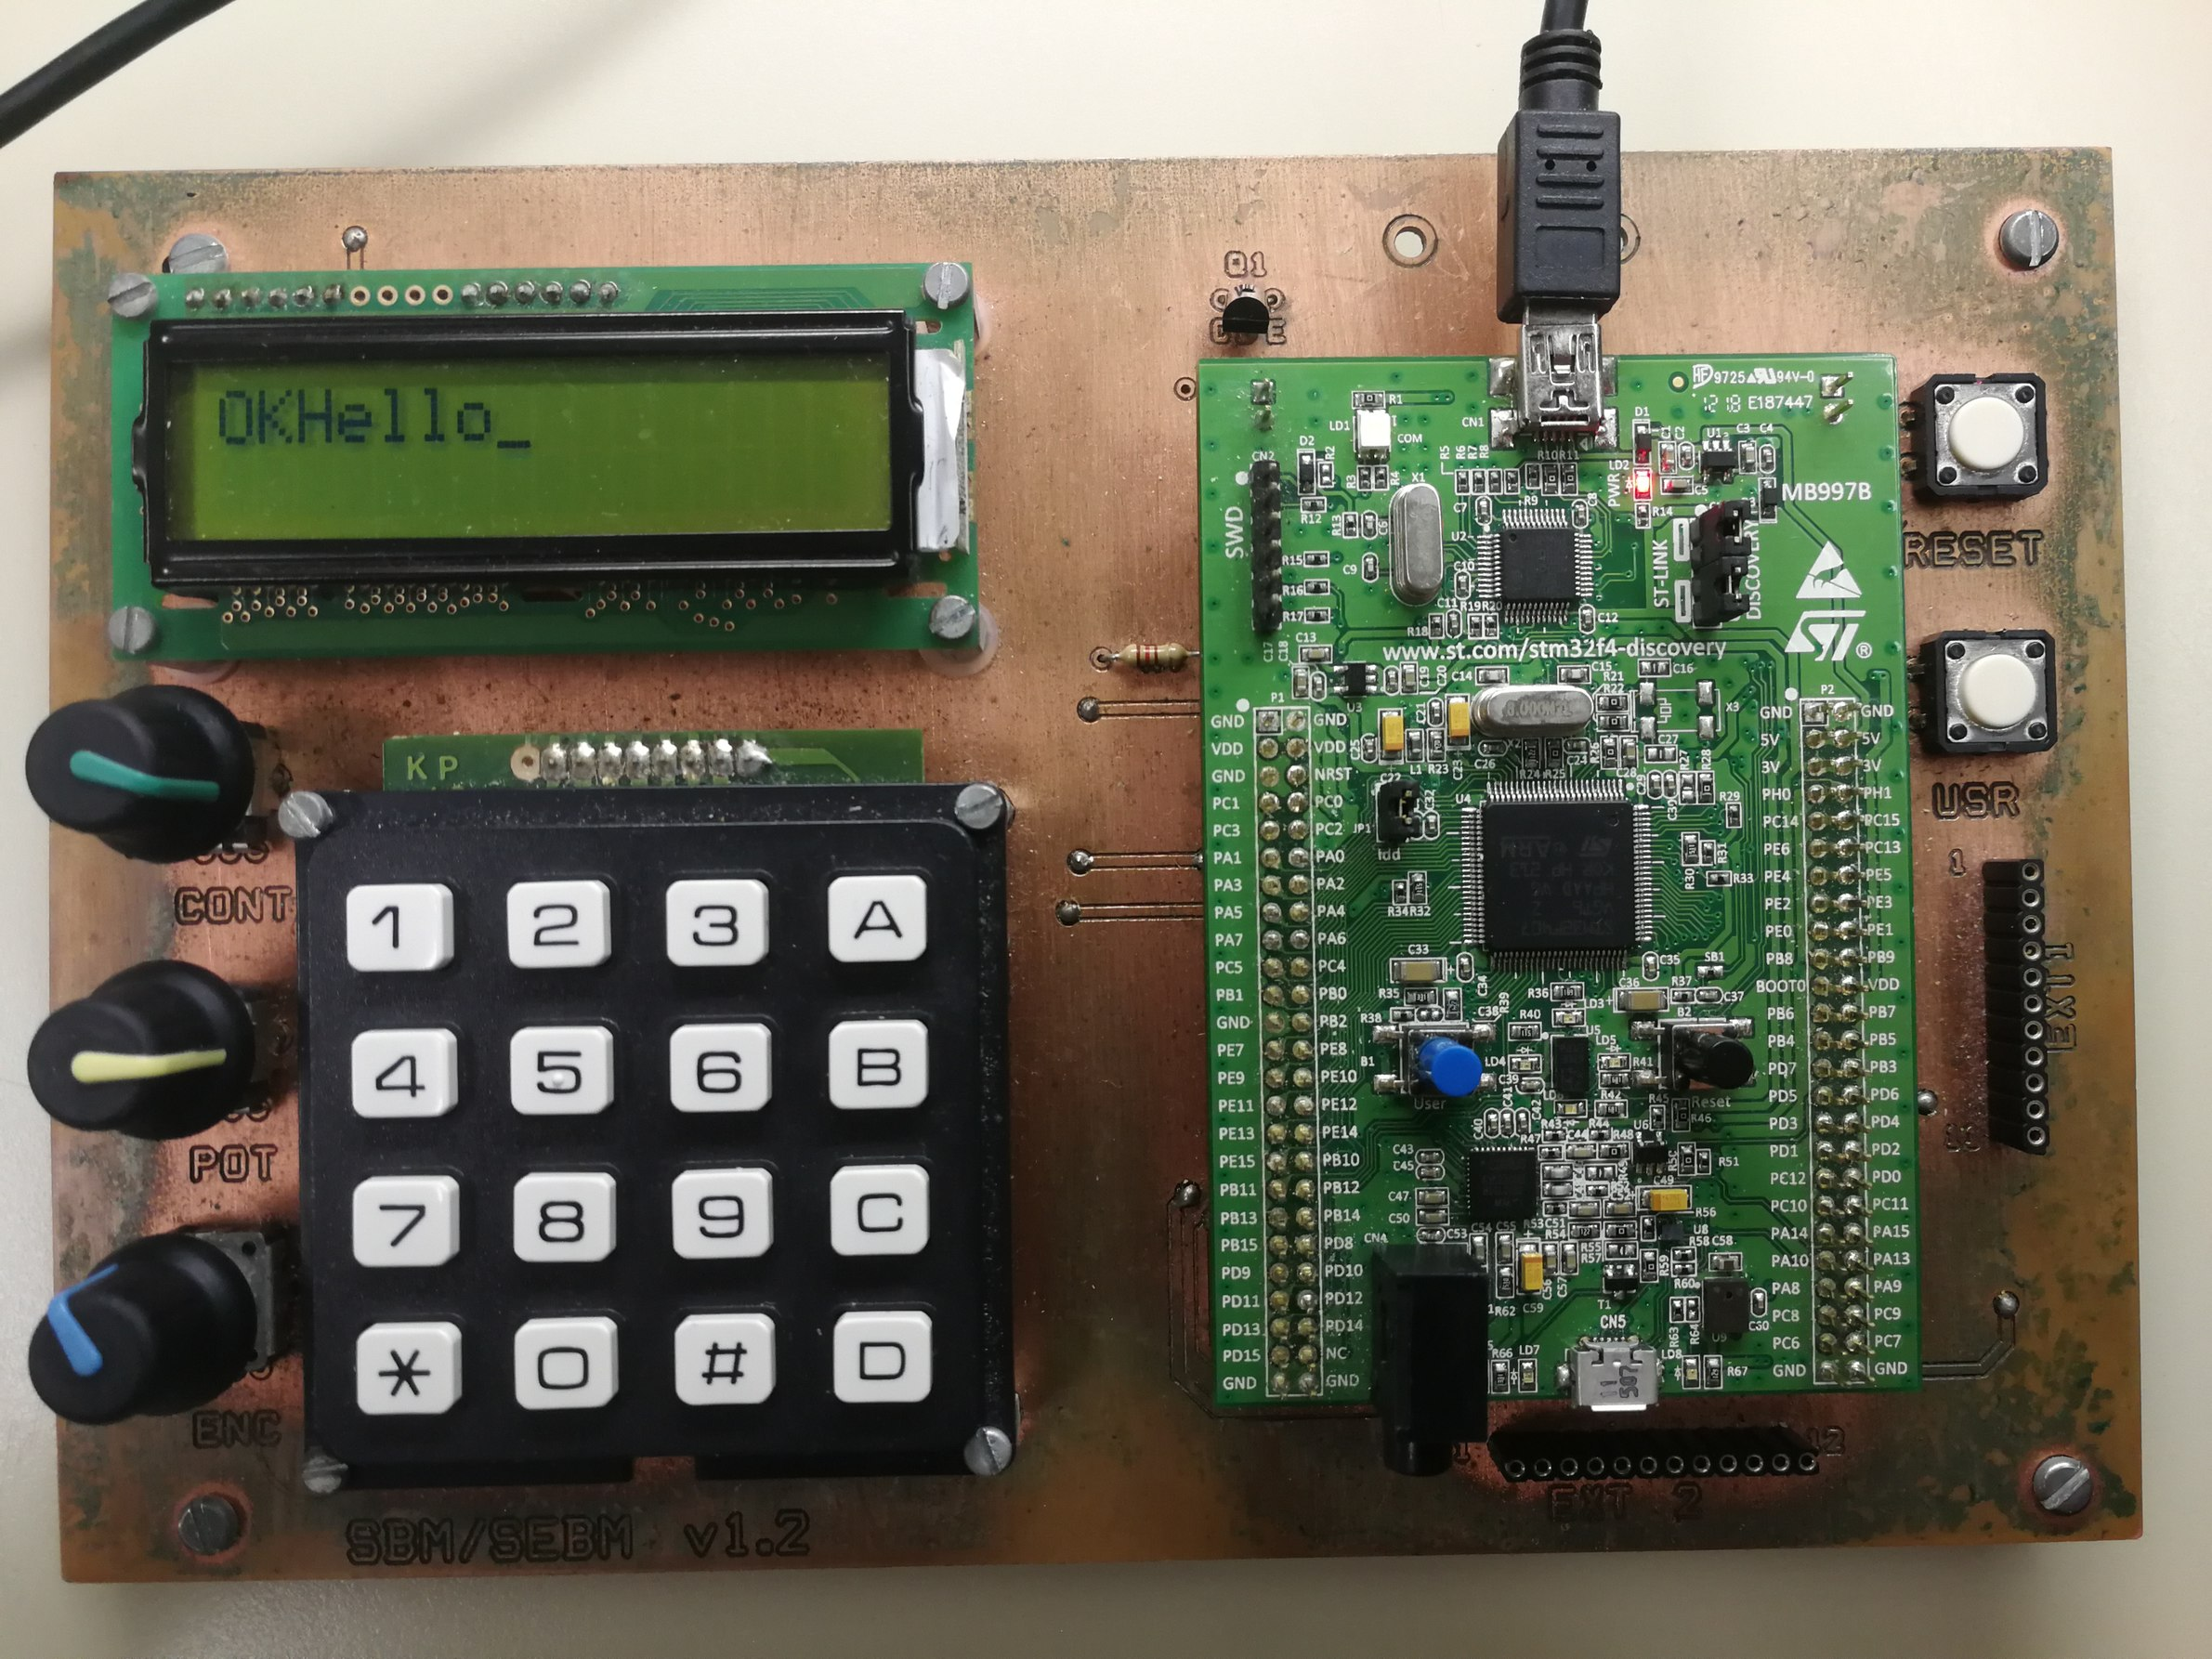
\includegraphics[width=1\columnwidth]{../photos/board/p2-hello}
  \end{center}
  \caption{ \label{fig:p2-board-hello} La placa després d'escriure \texttt{Hello} a l'LCD només inicialitzar-se. }
\end{figure}

Es demana ara que implementem la resta de funcions: \fname{LCD_ClearDisplay},
\fname{LCD_Config} i \fname{LCD_GotoXY}. Per brevetat es reprodueix la seva
implementació juntament amb els comentaris de documentació explicant la
funcionalitat que han de tenir (estudi previ):

%previ
\begin{minted}{c}
// Clear the LCD and set the cursor position at 0,0

void LCD_ClearDisplay(void) {
    lcdValue(0b00000001, 0);
    DELAY_US(1520);
}

// Configures the display
//     If Disp is TRUE turn on the display, if not, turns off
//     If Cursor is TRUE show the cursor, if not, hides it
//     If Blink is TRUE turn on blinking, if not, deactivate blinking

void LCD_Config(int32_t Disp, int32_t Cursor, int32_t Blink) {
    lcdValue(0b000001000 | (Disp ? BIT2 : 0) | (Cursor ? BIT1 : 0) | (Blink ? BIT0 : 0), 0);
    DELAY_US(40);
}

// Set the cursor at the given position
//    col: Columnn (0..LCD_COLUMNS-1)
//    row: Row     (0..LCD_ROWS-1)

void LCD_GotoXY(int32_t col, int32_t row) {
    uint32_t address = row * 0x40 + col;
    lcdValue(0b10000000 | (address & 0b1111111), 0);
    DELAY_US(40);
}
\end{minted}
\vskip -1em
%/previ

Un cop omplertes les tres funcions, s'indica que fem un programa senzill
que escrigui a la pantalla els noms dels dos membres del grup. En aquest
cas s'ha fet servir el cognom al segon lloc:

\begin{minted}{c}
void putNamesOnDisplay(void) {
    // Initialize the LCD
    LCD_Init();
    LCD_Backlight(TRUE);
    // Write things
    LCD_ClearDisplay();
    LCD_SendString("Alba");
    LCD_GotoXY(0, 1);
    LCD_SendString("Mendez");
    // No cursor
    LCD_Config(TRUE, FALSE, FALSE);
}
\end{minted}
\vskip -1em

El programa es carrega a la placa i s'obté el resultat esperat.
Se li ensenya al professor. Fins aquí, els canvis a \filename{lcd.c} i \filename{main.c}
conformen el \commit{557934f29e89773e5fbd82600321fcbfa0e852bf}.

\opcional

Addicionalment definirem i implementarem la funció \fname{LCD_CustomChar},
que, donat un string de 8 bytes, escriu aquests 8 bytes en la CGRAM
en l'espai indicat pel caràcter \mintinline{c}|pos| (de 0 a 7).
També es demana que, per evitar que crides a \fname{LCD_SendChar} posteriors
corrompin la CGRAM, en acabar la funció es torni a apuntar a la DDRAM.

La funció es defineix al header \filename{lcd.h}:

\begin{minted}{diff}
--- a/lcd.h
+++ b/lcd.h
@@ -51,6 +51,11 @@ void LCD_SendChar(char car);
 //     string: String to send
 void LCD_SendString(char *string);
 
+// Write a custom character to the CGRAM, and then goes to (0,0)
+// to prevent corruption of the CGRAM
+//     pos: Character to define (0..7)
+//     data: Buffer of 8 bytes to write
+void LCD_CustomChar(int32_t pos, uint8_t *data);
 
 #endif //_LCD_H
 
\end{minted}
\vskip -1em

I s'implementa a \filename{lcd.c} com segueix:

\begin{minted}{c}
// Write a custom character to the CGRAM, and then goes to (0,0)
// to prevent corruption of the CGRAM
//     pos: Character to define (0..7)
//     data: Buffer of 8 bytes to write

void LCD_CustomChar(int32_t pos, const uint8_t *data) {
    // Move to the corresponding CGRAM address
    uint32_t address = pos * 8;
    lcdValue(0b01000000 | (address & 0b111111), 0);
    DELAY_US(40);

    // Write each byte
    int32_t offset;
    for (offset = 0; offset < 8; offset++) {
        lcdValue(data[offset], 1);
        DELAY_US(40);
    }

    // Move back to DDRAM
    LCD_GotoXY(0, 0);
}
\end{minted}
\vskip -1em

Un cop implementada, per provar-la es modifica el programa que acabem
de fer per escriure un caracter amb forma de fletxa en la posició 2,
i es modifica la primera crida a \fname{LCD_SendString} per fer-lo servir:

\begin{minted}{diff}
--- a/main.c
+++ b/main.c
@@ -46,9 +46,21 @@ void putNamesOnDisplay(void) {
     // Initialize the LCD
     LCD_Init();
     LCD_Backlight(TRUE);
+    // Define a character
+    uint8_t e_acute [] = {
+        0b00000000,
+        0b00000001,
+        0b00000111,
+        0b00011111,
+        0b00000111,
+        0b00000001,
+        0b00000000,
+        0b00000000,
+    };
+    LCD_CustomChar(2, e_acute);
     // Write things
     LCD_ClearDisplay();
-    LCD_SendString("Alba");
+    LCD_SendString("Alba \x02\x02");
     LCD_GotoXY(0, 1);
     LCD_SendString("Mendez");
     // No cursor
\end{minted}
\vskip -1em

\begin{figure}
  \begin{center}
    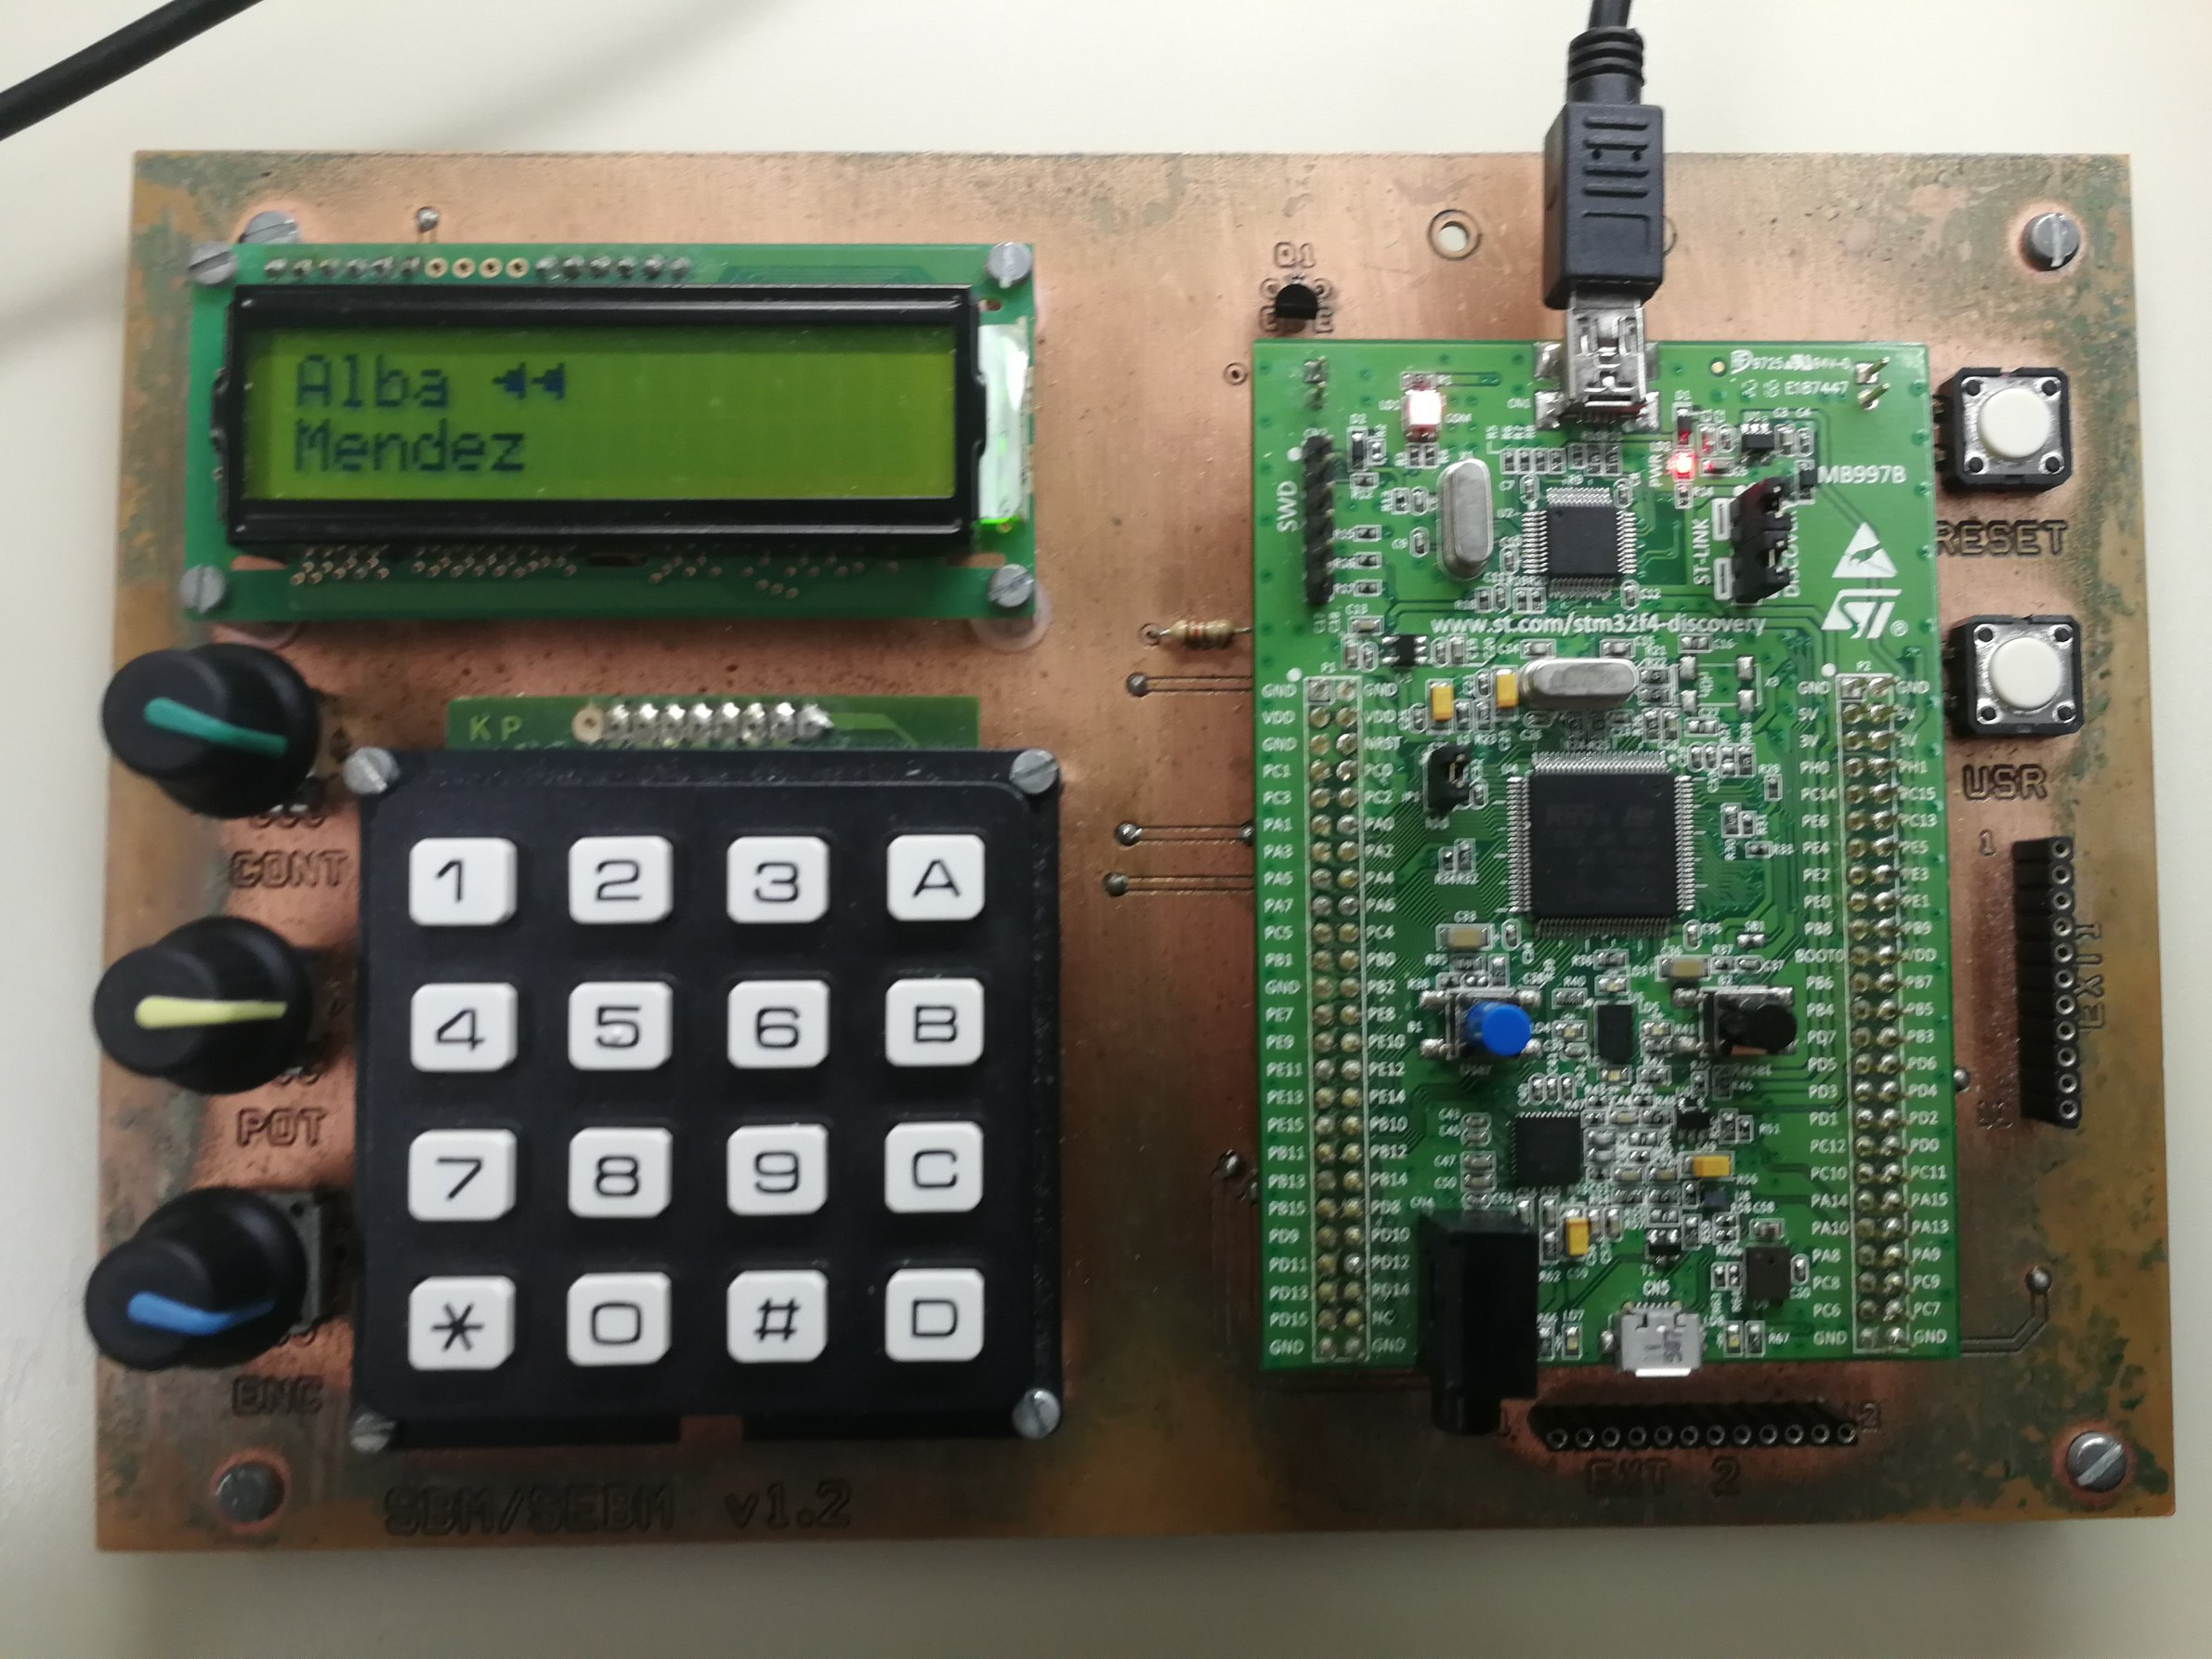
\includegraphics[width=1\columnwidth]{../photos/board/p2-names}
  \end{center}
  \caption{ \label{fig:p2-board-names} La placa mostrant nom i cognom a les dues fileres de l'LCD i un caràcter especial. }
\end{figure}

El codi es carrega a la placa i s'observa el resultat esperat (veure figura~\ref{fig:p2-board-names}).
Se li ensenya al professor. Els canvis a \filename{lcd.h}, \filename{lcd.c} i \filename{main.c}
conformen el \commit{468c685114db9e0fb23f0699b88b47d15234acdd}.


\section{Conclusió}

La pràctica s'ha realitzat sense problemes. S'ha trobat una càrrega conceptual gran,
especialment al principi, però després la implementació ha estat fàcil.
%FIXME: conclusion

\section{Ajustaments posteriors}

Durant la realització de pràctiques posteriors s'ha vist oportú millorar la qualitat del codi de \filename{util.c}
definint una macro anomenada \fname{SET_BITS}:

\begin{minted}{c}
#define SET_BITS(value, offset, nbits, bits) \
    value = ((value) & ~((BIT(nbits)-1) << (offset))) | ((bits) << (offset));
\end{minted}
\vskip -1em

Que manipula una quantitat de bits \mintinline{c}|nbits| començant pel bit més baix \mintinline{c}|offset|,
establint aquests bits al valor de \mintinline{c}|bits|. Amb això, el codi de \fname{GPIO_ModePushPull} esdevé:

\begin{minted}{c}
void GPIO_ModePushPull(GPIO_TypeDef *port, int32_t line) {
    line &= 0xF;

    // MODERy[1:0] -> 01 General purpose output mode
    SET_BITS(port->MODER, 2*line, 2, 0b01);

    // OTy -> 0 Push-pull output
    SET_BITS(port->OTYPER, line, 1, 0);

    // OSPEEDRy[1:0] -> 00 Speed 25MHz
    SET_BITS(port->OSPEEDR, 2*line, 2, 0b00);

    // PUPDRy[1:0] -> 00 No pull-up, no pull-down
    SET_BITS(port->PUPDR, 2*line, 2, 0b00);

    // ODRy -> 0 Low
    SET_BITS(port->ODR, line, 1, 0);
}
\end{minted}
\vskip -1em

També s'afegeix l'ordre \mintinline{c}|line &= 0xF;| al principi, que assegura que \mintinline{c}|line|
estigui entre 0 i 15 (per seguretat). Tot això és el \commit{da6142aab1f1cf2a6bafaa3d98a55262c5f985bb}.

També s'ha canviat l'ordre
en que es manipulen els registres, de forma que MODER es configuri al final, quan ODR
i la resta ja tenen els valors correctes. Així, el port passa d'un estat d'alta impedància
(entrada) directament a sortida baixa (0):

\begin{minted}{diff}
--- a/util.c
+++ b/util.c
@@ -19,9 +19,6 @@
 void GPIO_ModePushPull(GPIO_TypeDef *port, int32_t line) {
     line &= 0xF;
 
-    // MODERy[1:0] -> 01 General purpose output mode
-    SET_BITS(port->MODER, 2*line, 2, 0b01);
-
     // OTy -> 0 Push-pull output
     SET_BITS(port->OTYPER, line, 1, 0);
 
@@ -33,6 +30,10 @@ void GPIO_ModePushPull(GPIO_TypeDef *port, int32_t line) {
 
     // ODRy -> 0 Low
     SET_BITS(port->ODR, line, 1, 0);
+
+    // After everything is set up, switch mode
+    // MODERy[1:0] -> 01 General purpose output mode
+    SET_BITS(port->MODER, 2*line, 2, 0b01);
 }
 
 // Configure a GPIO line as open drain output, at the lowest speed,
\end{minted}
\vskip -1em

També, com a part de la pràctica P4, s'ha arreglat un bug important en la inicialització
de l'LCD. Això s'explica a la pàgina~\pageref{sub:p4-lcd}.
Aquests dos canvis conformen el \commit{d6babe86f524c875e7b5d9e93cf336c434c1b18c}.

Finalment, al \commit{ba419fc4317c5d8490daaeb8bcc1e137ea5c94cf} s'ha arreglat la definició
de \fname{LCD_CustomChar} per marcar l'argument com a \mintinline{c}|const|:

\begin{minted}{diff}
--- a/lcd.h
+++ b/lcd.h
@@ -55,7 +55,7 @@ void LCD_SendString(const char *string);
 // to prevent corruption of the CGRAM
 //     pos: Character to define (0..7)
 //     data: Buffer of 8 bytes to write
-void LCD_CustomChar(int32_t pos, uint8_t *data);
+void LCD_CustomChar(int32_t pos, const uint8_t *data);
 
 #endif //_LCD_H
 
\end{minted}
\vskip -1em

I el canvi corresponent a \filename{lcd.c}.

